%%%%%%%%%%%%%%%%%%%%%%%%%%%%%%%%%%%%%%%%%%  不使用 authblk 包制作标题  %%%%%%%%%%%%%%%%%%%%%%%%%%%%%%%%%%%%%%%%%%%%%%
%-------------------------------PPT Title-------------------------------------
\title{22-选讲专题:~机器学习方法简介}
%-----------------------------------------------------------------------------
%----------------------------Author & Date------------------------------------

%\author[\textrm{Jun\_Jiang}]{姜\;\;骏\inst{}} %[]{} (optional, use only with lots of authors)
%% - Give the names in the same order as the appear in the paper.
%% - Use the \inst{?} command only if the authors have different
%%   affiliation.
%\institute[BCC]{\inst{}%
\institute[Gain~Strong]{\inst{}%
%\vskip -20pt 北京市计算中心}
\vskip -20pt {\large 格致斯创~科技}}
\date[\today] % (optional, should be abbreviation of conference name)
{%	{\fontsize{6.2pt}{4.2pt}\selectfont{\textcolor{blue}{E-mail:~}\url{jiangjun@bcc.ac.cn}}}
\vskip 45 pt {\fontsize{8.2pt}{6.2pt}\selectfont{%清华大学\;\;物理系% 报告地点
	\vskip 5 pt \textrm{2023.04.22}}}
}

%% - Either use conference name or its abbreviation
%% - Not really information to the audience, more for people (including
%%   yourself) who are reading the slides onlin%%   yourself) who are reading the slides onlin%%   yourself) who are reading the slides onlineee
%%%%%%%%%%%%%%%%%%%%%%%%%%%%%%%%%%%%%%%%%%%%%%%%%%%%%%%%%%%%%%%%%%%%%%%%%%%%%%%%%%%%%%%%%%%%%%%%%%%%%%%%%%%%%%%%%%%%%

\subject{}
% This is only inserted into the PDF information catalog. Can be left
% out.
%\maketitle
\frame
{
%	\frametitle{\fontsize{9.5pt}{5.2pt}\selectfont{\textcolor{orange}{“高通量并发式材料计算算法与软件”年度检查}}}
\titlepage
}
%-----------------------------------------------------------------------------

%------------------------------------------------------------------------------列出全文 outline ---------------------------------------------------------------------------------
%\section*{}
%\frame[allowframebreaks]
%{
%  \frametitle{Outline}
%%  \frametitle{\textcolor{mycolor}{\secname}}
%  \tableofcontents%[current,currentsection,currentsubsection]
%}
%%在每个section之前列出全部Outline
%%类似的在每个subsection之前列出全部Outline是\AtBeginSubsection[]
%\AtBeginSection[]
%{
%  \frame<handout:0>%[allowframebreaks]
%  {
%    \frametitle{Outline}
%%全部Outline中,本部分加亮
%    \tableofcontents[current,currentsection]
%  }
%}

%-----------------------------------------------PPT main Body------------------------------------------------------------------------------------
\small
%\section{\rm{VASP~}软件中\rm{PAW~}计算的实现}
%\frame
%
%	\frametitle{\textrm{VASP}计算的特色}
%	相比于与普通的第一原理计算软件,\textrm{VASP}很好地平衡了计算效率和精度的问题,总的来说,\textrm{VASP}主要通过这几个特色保证了计算的高效能
%	\begin{itemize}
%	     \item 迭代与优化算法的多样性\\
%		     本质上电荷密度迭代 \textrm{\&\&} 体系总能量优化是相同的优化问题,采用了类似的算法\upcite{CMS6-15_1996,PRB54-11169_1996}:\\
%			\textcolor{blue}{\textrm{Pseudo-Newton、Conjugate-Gradient、Broyden~mix、damping-factor、RMM-DIIS}}
%	     \item 尽可能采用局域基(原子轨道基)函数:~\\
%		     \textcolor{blue}{\textrm{LREAL}}=\textcolor{red}{\textrm{.TRUE.}}\\
%			优化的投影函数也尽可能在实空间表示
%	     \item \textrm{PAW}原子数据集:\textcolor{blue}{优异的赝势}\upcite{PRB59-1758_1999}
%	\end{itemize}
%}
\frame
{
	\frametitle{第一原理计算与数据挖掘}
	\begin{itemize}
		\item 获取材料完整物性数据的成本,无论是通过实验手段还是计算模拟,代价都是比较高%的,虽然高通量第一原理计算自动流程和数据库解决了材料物性数据的获取问题,但是并未给出现有材料数据基础上的物性优化的方案,因此
		\item 利用数据挖掘技术,实现数据驱动的材料物性筛选、预测和提升的技术路线,有着特殊重要的意义。
		\item 机器学习\textrm{(Machine Learning, ML)}技术可以从大量数据中获得有价值的信息,尤其是面对高维复杂数据时,机器学习技术是确定数据间关系的有力的工具
	\end{itemize}
几十年来,机器学习的算法已经广泛应用于金融、导航控制、语言处理、游戏竞技、计算机可视化和生物信息学等领域。相反地,如果从非严格角度定义,任何计算机模拟人类智能的算法都可以划归为人工智能,并非一定要应用机器学习算法,也包括决策树、知识库、计算机逻辑等算法。近年来,机器学习领域的深度学习\textrm{(Deep Learning, DL)}异军突起,在很多领域都取得了很好的应用。深度学习是仿照生物神经网络\footnote{神经网络结构意味着输入输出之间允许有多个类似神经的网络层。}结构为主要代表的一种示类学习。
}

\frame
{
	\frametitle{机器学习}
机器学习是自动完成数据分析并提取数据关系的一类方法的统称,获取的数据关系可用于预测未知数据或辅助不确定条件下的决策过程
\begin{figure}[h!]
\centering
\vspace*{-0.1in}
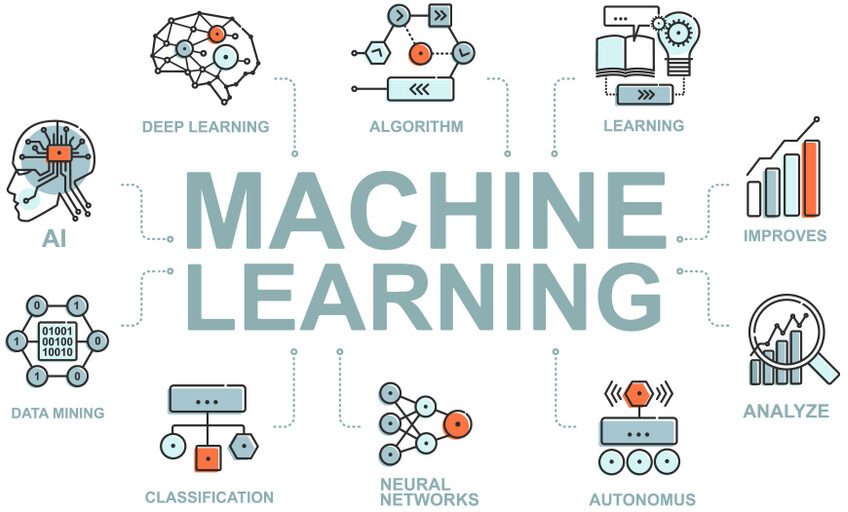
\includegraphics[height=2.3in,width=3.8in,viewport=0 0 630 390,clip]{Figures/Machine_Learning.jpg}
%\caption{\fontsize{7.2pt}{4.2pt}\selectfont{\textrm{人工智能与机器学习和深度学习的层次关系示意图.引自文献\cite{JPM2-032001_2019}}}}%
\label{Machine-Learning}
\end{figure}
}

\frame
{
	\frametitle{人工智能和机器学习的层次关系}
传统定义界定的机器学习,是指无须借助解析程序,直接依靠数据来提升任务处理的性能,自从1950年代统计学、计算科学与技术和神经科学的发展,机器学习的研究发展到了更广泛的人工智能\textrm{(Artificial Intelligence, AI)}领域。%图\ref{AI-ML}表明了人工智能和机器学习的层次关系。
\begin{figure}[h!]
\centering
\vspace*{-0.1in}
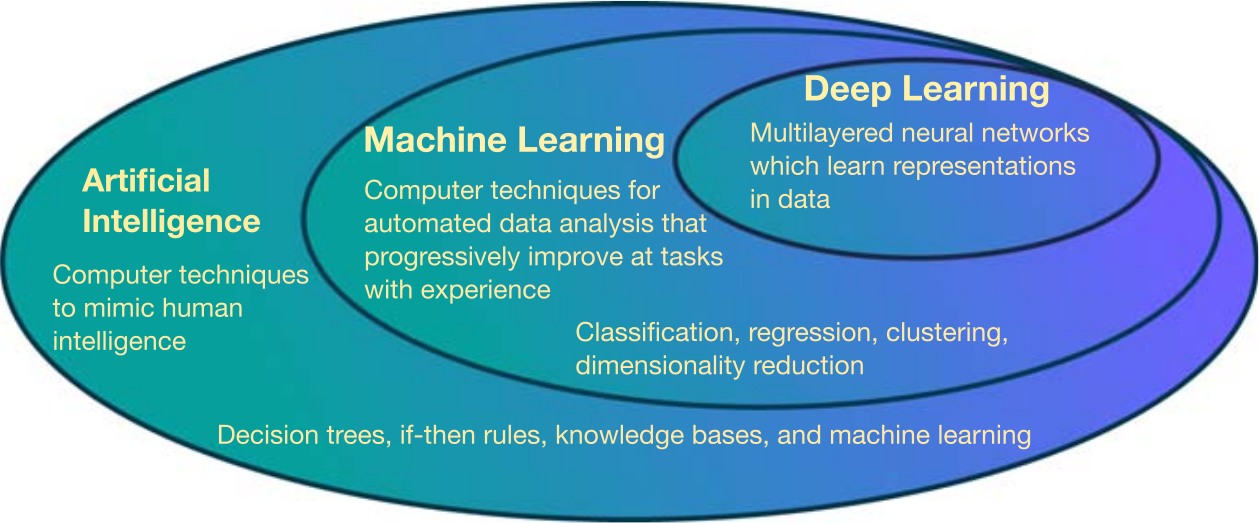
\includegraphics[height=1.7in,width=4.0in,viewport=0 0 1275 550,clip]{Figures/Hierarchical_description_AI_ML_DL.png}
\caption{\fontsize{7.2pt}{4.2pt}\selectfont{\textrm{人工智能与机器学习和深度学习的层次关系示意图.引自文献\cite{JPM2-032001_2019}}}}%
\label{AI-ML}
\end{figure}
}

\frame
{
	\frametitle{机器学习问题的种类}
}
}
